%%%%%%%%%%%%%%%%%%%%%%%%%%%%%%%%%%%%%%%%%%%%%%%%%%%%%%%%%%%%%%%%%%%%%%%%%%%%%%%%
% ELEN E6885 Final Report -- DRAFT
% Use with Overleaf's ICML template: replace the template's example .tex with this file,
% and upload  references.bib, figures/*.pdf, tables/*.tex  (see report/README.md).
% Lines marked  %TODO  still need results or your decision.
%%%%%%%%%%%%%%%%%%%%%%%%%%%%%%%%%%%%%%%%%%%%%%%%%%%%%%%%%%%%%%%%%%%%%%%%%%%%%%%%
\documentclass{article}
\usepackage{microtype}
\usepackage{graphicx}
\usepackage{subcaption}
\usepackage{booktabs}
\usepackage{hyperref}
\usepackage{amsmath,amssymb,amsthm}
\usepackage{algorithm}
\usepackage{algorithmic}
\newcommand{\theHalgorithm}{\arabic{algorithm}}
% Use the year of the template Overleaf gives you (icml2025 / icml2026):
\usepackage[accepted]{icml2025}
\newtheorem{proposition}{Proposition}

\icmltitlerunning{Do Fairness Constraints Survive Distribution Shift?}

\begin{document}

\twocolumn[
\icmltitle{Do Fairness Constraints Survive Distribution Shift?\\
           Constrained Reinforcement Learning for Traffic Signal Control}
\begin{icmlauthorlist}
\icmlauthor{Your Name}{cu}   %TODO your name
\end{icmlauthorlist}
\icmlaffiliation{cu}{Department of Electrical Engineering, Columbia University, New York, USA}
\icmlcorrespondingauthor{Your Name}{uni@columbia.edu}   %TODO
\icmlkeywords{Reinforcement Learning, Constrained MDP, Traffic Signal Control, Fairness, Robustness}
\vskip 0.3in
]
\printAffiliationsAndNotice{}

%===============================================================================
\begin{abstract}
Reinforcement learning (RL) traffic signal controllers are trained to minimize \emph{average}
delay, and so are classical throughput-optimal rules such as Max-Pressure.
We show, analytically and in simulation, that this objective can starve low-demand approaches:
in a simple fluid model the average-delay-optimal policy makes the side-road maximum wait
grow as $\lambda_2^{-1/2}$ while the mean delay goes to zero, and in SUMO Max-Pressure leaves
side-road vehicles waiting up to 378\,s although its mean delay is only 15.5\,s.
We cast fairness as an explicit constraint on the maximum waiting time and solve it with
Lagrangian PPO. On a single intersection it meets the target violation rate
(5.4\% vs.\ a 5\% target, down from 11.3\% for PPO, $p<0.001$) and cuts the maximum delay by
22\% at a cost of 1.7\,s mean delay, whereas reward shaping and structural (max-red)
constraints are either ineffective or highly sensitive to their tuning.
We then ask whether the guarantee \emph{survives distribution shift}: under a demand surge the
violation rate of every method, including ours, rises to 23--51\%, and detector failures
degrade it further. Domain randomization over the feasible demand region reduces the
violation rate under shift by 40\% ($p=0.02$), but an expected constraint over a training
distribution does not hold on every scenario, pointing to robust constraints as the open problem.
Code and all results: \url{https://github.com/Ca1He/traffic-rl}.
\end{abstract}

%===============================================================================
\section{Introduction}
Signalized intersections are a textbook sequential decision problem, and deep RL controllers
now routinely outperform fixed-time plans in simulation
\cite{WeiZYL18,WeiCZWGXL19,WeiXZZZCZZXL19,ZhengXZFWZLXL19}. Almost all of them optimize an
\emph{average} efficiency signal---cumulative waiting time, queue length or pressure.
Averages hide distributions: a controller can keep the main road flowing and the mean delay
low while a handful of side-road drivers wait for minutes (Fig.~\ref{fig:teaser}).
Such starvation is not only unfair; drivers who wait too long run red lights, and
practitioners impose maximum-red rules for exactly this reason.

Fairness in RL signal control has been addressed by reshaping the reward
\cite{RaeisL21,YanZBB20,YeDWZWC23}, by multi-objective welfare functions \cite{SiddiqueWZ20},
and recently by constraints \cite{HaydariAZC25,SatheeshP25}. Separately, RL controllers are
known to be brittle to sensor failures and demand changes \cite{RodriguesA19,TanSS20,AultS21,MeiLSW23}.
These two lines have not met: a fairness guarantee obtained in training is only useful if it
still holds when the traffic or the sensors change, and \emph{no prior work evaluates this}.

\textbf{Contributions.}
(1) A simple fluid-model proposition showing that average-delay-optimal control starves
low-demand approaches, with the maximum wait scaling as $\lambda_2^{-1/2}$, while the price of
a max-wait constraint is bounded independently of $\lambda_2$; we confirm the predicted trend
in SUMO (Sec.~\ref{sec:prop}).
(2) An outcome constraint on the maximum waiting time solved with Lagrangian PPO, compared
under one protocol with reward-shaping and structural (max-red) fairness, on a single
intersection and a 2$\times$2 grid, where we show that the constraint must use the
\emph{local} wait each signal can control (Sec.~\ref{sec:method}, \ref{sec:exp}).
(3) The first evaluation of whether fairness constraints survive demand shift and detector
dropout, and of domain randomization over the \emph{feasible} operating region as a remedy
(Sec.~\ref{sec:robust}).

%===============================================================================
\section{Background and Related Work}
\textbf{Classical control.} Webster's fixed-time plan sets the cycle to
$C_0=(1.5L+5)/(1-Y)$ and splits green in proportion to critical flow ratios \cite{Webster58}.
Max-Pressure serves the phase with the largest upstream-minus-downstream queue and is
throughput-optimal \cite{Varaiya13,TassiulasE92}; stability, however, says nothing about how
long an individual vehicle waits.

\textbf{RL for signal control.} IntelliLight \cite{WeiZYL18}, PressLight \cite{WeiCZWGXL19},
CoLight \cite{WeiXZZZCZZXL19} and FRAP \cite{ZhengXZFWZLXL19} use DQN variants with
efficiency rewards; \citet{ZhangWSLDW22} show that well-designed pressure states make even
simple controllers strong. Surveys and benchmarks: \cite{WeiZGL19survey,AultS21}.

\textbf{Constrained RL.} A constrained MDP (CMDP) maximizes
$J_r(\pi)=\mathbb{E}_\pi[\sum_t r_t]$ subject to $J_c(\pi)\le d$ \cite{Altman99}.
Lagrangian methods alternate policy improvement on $r-\lambda c$ with dual ascent on
$\lambda\ge 0$ \cite{TesslerMM19,RayAA19,StookeAA20}; CPO enforces the constraint per update
\cite{AchiamHTA17}.

\textbf{Fairness and robustness in RL signal control.} \citet{RaeisL21} penalize the
squared waiting time in the reward and report tail metrics; \citet{SiddiqueWZ20} optimize a
Gini welfare over per-lane waits. Closest to us, FAirLight \cite{HaydariAZC25} constrains
fairness and emissions with off-policy max-entropy RL, and MAPPO-LCE \cite{SatheeshP25}
applies Lagrangian MAPPO to \emph{structural} rules (max green, phase skips). Robustness to
surges, incidents, sensor noise and missing data was studied by
\cite{RodriguesA19,TanSS20,MeiLSW23,ShiDLC23}, without fairness.
\textbf{Our difference:} we constrain the \emph{outcome} (max wait) rather than the signal
program, compare it head-to-head with shaping and structural constraints, and test whether
the constraint---not just efficiency---survives distribution shift.
%TODO read FAirLight full text (DOI 10.1145/3676169) and sharpen this sentence if needed.

%===============================================================================
\section{Approach}\label{sec:method}
\textbf{MDP.} Every $\Delta t=5$\,s the agent observes the current phase (one-hot), a
min-green flag and, for each incoming lane, the normalized density and queue from a loop
detector; it selects one of four green phases (3\,s yellow on change, 10\,s min green and a
60\,s max green that we enforce ourselves since sumo-rl ignores it). The reward is the
decrease in cumulative waiting time \cite{sumorl}.

\textbf{Fairness constraint.} Let $W_t$ be the largest accumulated waiting time of any vehicle
on an incoming lane. The per-step cost is $c_t=\mathbb{1}[W_t>T]$ with $T=90$\,s, and we
require the \emph{violation rate} $J_c(\pi)=\mathbb{E}_\pi[\frac1H\sum_t c_t]\le d=0.05$:
at most 5\% of decision steps may have a vehicle waiting longer than $T$.
In a network a vehicle's accumulated wait includes delay suffered upstream, which the local
signal cannot influence; there we use the wait accumulated \emph{since the vehicle reached
this intersection}. With trip-level waits the local constraint was unsatisfiable and
$\lambda$ grew without bound (Sec.~\ref{sec:grid}).

\textbf{Lagrangian PPO} (Alg.~\ref{alg:lag}). We run PPO \cite{SchulmanWDRK17} with GAE
\cite{SchulmanMLJA16} on the penalized reward $r_t-\lambda c_t$ with a single critic, as in
RCPO \cite{TesslerMM19}, and update $\lambda$ once per rollout by projected dual ascent.
The dual step is far slower than the many PPO minibatch updates (two time scales).
A step size of $\eta=0.05$ overshot ($\lambda\approx1.1$, mean delay doubled); we use $\eta=0.01$.

\begin{algorithm}[t]
\caption{Lagrangian PPO for the max-wait constraint}\label{alg:lag}
\begin{algorithmic}
\STATE \textbf{input:} threshold $T$, target $d$, dual step $\eta$, $\lambda\gets0$
\FOR{each rollout of 720 steps (one hour of traffic)}
  \STATE collect $(s_t,a_t,r_t,c_t)$ with $c_t=\mathbb{1}[W_t>T]$
  \STATE PPO update (10 epochs) on penalized rewards $r_t-\lambda c_t$
  \STATE $\hat J_c\gets\frac{1}{720}\sum_t c_t$;\quad
         $\lambda\gets\mathrm{clip}\big(\lambda+\eta(\hat J_c-d),\,0,\,\lambda_{\max}\big)$
\ENDFOR
\end{algorithmic}
\end{algorithm}

\textbf{Sensing and domain randomization.} All controllers, including Max-Pressure, read
traffic through the same detector model: Gaussian noise and dropout with probability $p$
(redrawn every step, or a fixed set of failed detectors per episode). For domain
randomization (DR) \cite{TobinFRSZA17} each training episode draws a new demand (per-approach
rates $\sim U[100,850]$\,veh/h, half the episodes with a change point) and $p\sim U[0,0.3]$.
We keep only demands with Webster flow ratio $Y\le0.85$: 12\% of unfiltered draws are
oversaturated ($Y>1$), where no controller can meet any wait constraint, and in our first DR
runs these samples drove $\lambda$ up without bound.

%-------------------------------------------------------------------------------
\subsection{Why average-optimal control starves the side road}\label{sec:prop}
Consider a fluid model with a main road (rate $\lambda_1$, utilization
$\rho=\lambda_1/\mu$) and a side road (rate $\lambda_2\ll\lambda_1$). Serving the side road
costs a lost time $L$ per switch. A policy serves the main road and every $T$ seconds makes an
excursion of length $\tau\approx2L$ to clear the side road. Each excursion adds main-road delay
$K=\lambda_1\tau^2/(2(1-\rho))=2\lambda_1L^2/(1-\rho)$; side-road vehicles wait up to $T$,
contributing $\lambda_2T^2/2$. The total delay rate is $J(T)=K/T+\lambda_2T/2$.

\begin{proposition}\label{prop:starve}
(a) The average-delay-optimal period is
$T^*=2L\sqrt{\lambda_1/((1-\rho)\lambda_2)}$, so the maximum side-road wait $W_2^*=T^*$
diverges as $\lambda_2/\lambda_1\to0$ or $\rho\to1$, while the mean delay per vehicle
$\sqrt{2K\lambda_2}/(\lambda_1+\lambda_2)\to0$.
(b) Enforcing $W_2\le T_{\max}<T^*$ increases the mean delay per vehicle by at most
$2L^2/((1-\rho)T_{\max})$, independently of $\lambda_2$.
\end{proposition}
\emph{Proof sketch.} $J$ is convex with $J'(T^*)=0$ giving (a). For (b) the constrained
optimum is $T_{\max}$ and $J(T_{\max})-J(T^*)\le K/T_{\max}$; divide by $\lambda_1+\lambda_2\ge\lambda_1$.
Full proof in the supplement. The result formalizes a classical observation about priority
service \cite{Kleinrock76}; we present it as an illustration, not a new theorem.

Fig.~\ref{fig:prop} sweeps the side-road demand in SUMO with the main road fixed at
800\,veh/h. Max-Pressure, which is efficiency-oriented, lets the side-road maximum wait grow
from 281\,s to 747\,s as the side demand falls from 400 to 25\,veh/h, while its mean delay
\emph{improves} from 23.7\,s to 10.6\,s (log--log slope $-0.36$ vs.\ $-0.5$ predicted; the
fluid model ignores stochastic arrivals and min-green). Webster, which splits green by
demand, shows the opposite trend.

%===============================================================================
\section{Experiments}\label{sec:exp}
\textbf{Setup.} SUMO 1.28 \cite{LopezBBEFHLRWW18} via sumo-rl \cite{sumorl}; a 4-arm
intersection with two lanes per arm (through+right, left), 3600\,s episodes and Poisson-like
arrivals (60/20/20\% through/left/right). Demands: \emph{balanced} (500\,veh/h per arm),
\emph{asym} (main 800, side 200) and \emph{surge} (asym, then a 20-min side-road surge to
700 with the main road at 500, then asym). Saturation flows for Webster were measured in
SUMO (1630 / 1120\,veh/h for through / left lanes). PPO and DQN come from Stable-Baselines3
\cite{RaffinHGKED21} (hyperparameters in the supplement); RL methods are trained for 300k
steps with 5 seeds (3 for ablations). Every metric uses \emph{all} vehicles---including
those still in the network or not yet inserted at the end of the episode---since dropping
them would hide exactly the starved vehicles. We report mean $\pm$ std over training seeds
of 5 evaluation episodes each, and Welch's $t$-test \cite{HendersonIBPPM18}. All runs take
about 6 CPU-hours on a laptop.

\begin{figure}[t]
\centering
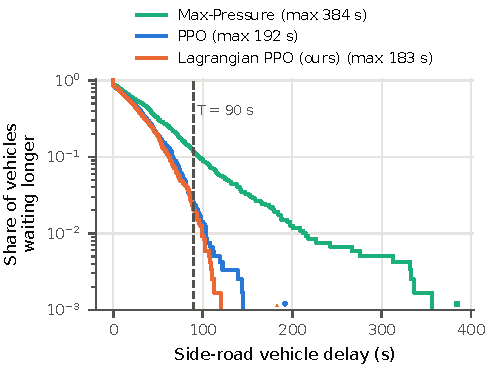
\includegraphics[width=\columnwidth]{figures/fig1_teaser.pdf}
\caption{Share of side-road vehicles that waited longer than $x$ (asym, 3 episodes, log scale).
Max-Pressure has the lowest mean delay but a long tail; Lagrangian PPO cuts the tail near $T=90$\,s.}
\label{fig:teaser}
\end{figure}

\begin{table*}[t]
\centering
\caption{Single intersection. Mean $\pm$ std over 5 training seeds (RL) or 5 evaluation episodes
(baselines). Violation rate: share of decision steps with a vehicle waiting $>90$\,s (target 0.05).
All RL policies were trained on asym only; surge is unseen. Best value per column in bold.}
\label{tab:main}
\small
\input{tables/main_table.tex}
\end{table*}

\textbf{Average-optimal control is unfair.} (Tab.~\ref{tab:main}) On asym, Max-Pressure has the
lowest mean delay (15.5\,s) but the worst max delay among adaptive methods (378\,s) and a
36\% violation rate. Queue and pressure rewards make RL starve the side road completely
(violation rate 0.93 / 0.97, max delay $>$1000\,s; Tab.~\ref{tab:ablation}); the
waiting-time reward is better but still violates in 11\% of steps.

\textbf{The constraint is met precisely and cheaply.} Lagrangian PPO reaches a 5.4\% violation
rate (target 5\%; PPO 11.3\%, $p=0.0009$), reduces the max delay from 194\,s to 152\,s
($p=0.006$) and raises the mean delay by 1.7\,s. Fig.~\ref{fig:training} shows $\lambda$
settling near 0.19. Reward shaping \cite{RaeisL21} is hard to tune: $\alpha=5$ still violates
in 14\% of steps and $\alpha=20$ destabilizes training (79\%). A fixed penalty works only near
the $\lambda$ that the dual update finds automatically; ten times larger doubles the mean delay.
A structural max-red constraint with $R=90$\,s performs comparably on max delay but costs
3.3\,s more mean delay ($p=0.05$), and $R=60$\,s makes the controller collapse (mean delay 149\,s).
Fig.~\ref{fig:tradeoff} summarizes the trade-off.

\begin{figure}[t]
\centering
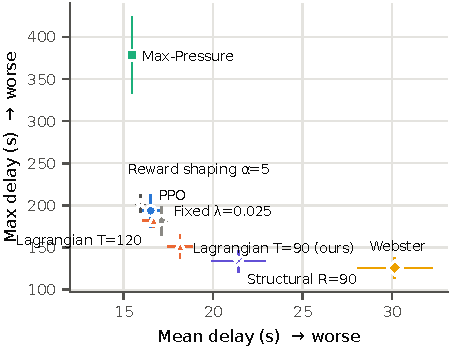
\includegraphics[width=\columnwidth]{figures/fig3_tradeoff.pdf}
\caption{Mean vs.\ max delay on asym (mean $\pm$ std). Lower-left is better.}
\label{fig:tradeoff}
\end{figure}

\begin{table}[t]
\centering
\caption{Ablations on asym (PPO, violation rate at $T=90$\,s; 5 seeds for default and ours, 3 otherwise).}
\label{tab:ablation}
\resizebox{\columnwidth}{!}{\input{tables/ablation_table.tex}}
\end{table}

%-------------------------------------------------------------------------------
\subsection{Does the constraint survive distribution shift?}\label{sec:robust}
\textbf{Demand shift.} On the unseen surge demand every method breaks the 5\% target
(Tab.~\ref{tab:main}, right): Webster, tuned to the average demand, reaches 51\%,
Max-Pressure 44\%, PPO 28\% and Lagrangian PPO 23\%---no longer significantly better than PPO
($p=0.16$). A constraint satisfied in training gives no guarantee after a shift.

\textbf{Detector faults.} Sensor faults erode the constraint as well (Fig.~\ref{fig:robust}).
On the training demand the violation rate of Lagrangian PPO rises from 4.5\% to 9.9\% when each
detector fails with $p=0.3$ at every step, to 16\% under Gaussian noise ($\sigma=0.1$) and to
21\% when 20\% of the detectors fail for the whole episode---the hardest condition for every
method. Interestingly, Max-Pressure becomes \emph{less} unfair under dropout (36\%$\to$28\%):
missing readings break its persistent preference for the main road.

\textbf{Domain randomization.} Training over random demands (per-approach rates
$U[100,850]$, half with a change point) without filtering did not converge: 12\% of the draws
are oversaturated, no policy can meet the constraint there, and $\lambda$ grew linearly
(to 2.8 after 800k steps) while the mean delay rose to 26\,s. Restricting the draws to the
feasible region ($Y\le0.85$) fixes this ($\lambda\approx0.3$--$0.8$, training violation rate
4--11\%). The resulting policy is far more robust: on the unseen surge its violation rate is
14.0\% vs.\ 23.4\% for Lagrangian PPO ($p=0.02$) and 28.4\% for PPO ($p<0.001$), its max delay
drops from 271\,s to 203\,s ($p=0.04$), and it stays below every non-DR method under all
dropout levels. Also randomizing the detectors brings no further gain ($p=0.25$).
The price is that on asym itself it violates in 12.7\% of steps instead of 5.4\%.
This exposes a structural limit: the Lagrangian enforces the violation rate \emph{in
expectation over the training distribution}, so light scenarios end up far below $d$ and
heavy ones above it. Neither training regime yields a per-scenario guarantee; that requires
a worst-case or distributionally robust constraint.

\begin{figure*}[t]
\centering
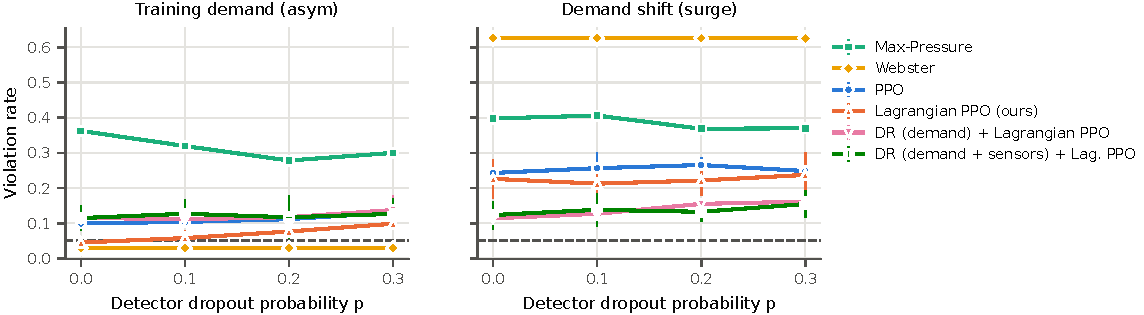
\includegraphics[width=\textwidth]{figures/fig4_robustness.pdf}
\caption{Violation rate under detector dropout on the training demand (left) and on the unseen
surge demand (right); mean $\pm$ std over training seeds, 3 episodes each. Dashed: target $d=0.05$.
Only Webster (tuned to asym, sensor-free) meets the target in training and it fails worst under shift;
domain randomization (DR) gives the lowest violation rate under shift at every dropout level.}
\label{fig:robust}
\end{figure*}

%-------------------------------------------------------------------------------
\subsection{2$\times$2 grid}\label{sec:grid}
We train one parameter-shared PPO policy for all four intersections (IPPO
\cite{deWittGMMTSW20,YuVVGWBW22}) for 1.5M steps, with E--W as the main road (600\,veh/h) and
N--S as the side road (150\,veh/h). With the trip-level wait as cost, $\lambda$ kept rising
(0.55 after 1.5M steps, violation rate stuck at 11\%) because downstream signals were charged
for upstream delay; with the local wait it converges ($\lambda\approx0.09$).
Lagrangian IPPO meets the target (4.6\% vs.\ 6.1\% for IPPO and 14.9\% for Max-Pressure) at
+0.6\,s mean delay (Tab.~\ref{tab:grid}). The gain is smaller than on one intersection
because unconstrained IPPO is already fairer here; under surge both exceed the target again.

\begin{table}[t]
\centering
\caption{2$\times$2 grid (local violation rate, $T=90$\,s). RL: 3 seeds.}
\label{tab:grid}
\resizebox{\columnwidth}{!}{\input{tables/grid_table.tex}}
\end{table}

%===============================================================================
\section{Conclusion}
Minimizing average delay starves low-demand approaches, provably in a fluid model and
visibly in simulation. An explicit max-wait constraint solved with Lagrangian PPO enforces a
chosen violation rate at a small efficiency cost and without the tuning fragility of reward
shaping or structural rules. However, the guarantee does not transfer: under a demand surge
all methods, including the constrained one, violate the target several-fold, and detector
faults make it worse. Domain randomization restricted to feasible demand cuts the violation
under shift by 40\%, but an expectation constraint cannot give per-scenario guarantees.
\textbf{Limitations.} One simulator, a single intersection and a 2$\times$2 grid, synthetic
demand, random rather than adversarial sensor faults \cite{ZhangCXLLBH20}, and a constraint on
the expected violation rate rather than a hard per-episode bound. Future work: robust or
distributionally robust constraints, larger networks and real demand data.

%===============================================================================
\bibliography{references}
\bibliographystyle{icml2025}

\section*{Statement of Contributions}
This is a single-author project. The author designed the study, implemented the environment
wrappers, baselines, Lagrangian PPO and evaluation pipeline, ran all experiments, derived
Proposition~\ref{prop:starve}, and wrote the report.
%TODO Check the course policy on AI assistance and, if required, disclose it here.

%===============================================================================
\newpage
\appendix
\onecolumn
\section{Supplementary material}
\textbf{Full proof of Proposition~\ref{prop:starve}.}
\emph{Model.} Two approaches with deterministic fluid arrivals $\lambda_1$ (main) and
$\lambda_2\ll\lambda_1$ (side), saturation flow $\mu$, $\rho=\lambda_1/\mu<1$, lost time $L$
per switch. Policy class $\Pi_T$: serve the main road by default; every $T$ seconds make an
excursion that clears the side-road queue and switches back. For small $\lambda_2$ the
excursion lasts $\tau\approx2L$ (the side-road service time $\lambda_2T/\mu$ is negligible).
\emph{Main-road delay.} During an excursion the main-road queue grows to $\lambda_1\tau$ and
then drains at rate $\mu-\lambda_1$; the area of this triangle is
$K=\tfrac12\lambda_1\tau\cdot\tau\mu/(\mu-\lambda_1)=\lambda_1\tau^2/(2(1-\rho))=2\lambda_1L^2/(1-\rho)$.
\emph{Side-road delay.} Side vehicles arrive uniformly over the cycle and wait until the next
excursion: total delay $\lambda_2T^2/2$ per cycle, and the vehicle arriving just after an
excursion waits $\approx T$, so the maximum side wait is $W_2=T$.
\emph{(a)} The delay rate $J(T)=K/T+\lambda_2T/2$ is convex on $T>0$; $J'(T)=-K/T^2+\lambda_2/2=0$
gives $T^*=\sqrt{2K/\lambda_2}=2L\sqrt{\lambda_1/((1-\rho)\lambda_2)}$, which diverges as
$\lambda_2/\lambda_1\to0$ or $\rho\to1$. At $T^*$ both terms are equal, $J(T^*)=\sqrt{2K\lambda_2}$,
and the mean delay per vehicle $J(T^*)/(\lambda_1+\lambda_2)\to0$ as $\lambda_2\to0$.
\emph{(b)} For $T_{\max}<T^*$, convexity puts the constrained minimizer at $T_{\max}$, and
$J(T_{\max})-J(T^*)=K/T_{\max}+\lambda_2T_{\max}/2-\sqrt{2K\lambda_2}$. Since
$\lambda_2T_{\max}/2<\lambda_2T^*/2=\sqrt{2K\lambda_2}/2$, the last two terms sum to a negative
number, so the increase is at most $K/T_{\max}$; per vehicle,
$K/(T_{\max}(\lambda_1+\lambda_2))\le2L^2/((1-\rho)T_{\max})$. $\square$
\emph{Numbers for asym:} $L\approx5$\,s, $\rho\approx0.39$, $T^*\approx26$\,s and a price-of-fairness
bound of $0.9$\,s/veh for $T_{\max}=90$\,s. The fluid model ignores min-green, stochastic
arrivals and left-turn phases, so it predicts scaling, not absolute waits.
\textbf{Hyperparameters.} PPO: lr $3\cdot10^{-4}$, 720 steps per rollout, batch 180, 10 epochs,
$\gamma=0.99$, GAE $\lambda=0.95$, clip 0.2, entropy 0.01, MLP $[64,64]$.
DQN: lr $10^{-3}$, buffer 50k, batch 64, target update 500, $\epsilon$: 1$\to$0.02 over 20\%.
Lagrangian: $d=0.05$, $\eta=0.01$, $\lambda_{\max}=20$. Grid PPO: batch 720.
\textbf{Reproduction.} \texttt{README.md} in the repository lists one command per table and figure.

\begin{figure}[h]
\centering
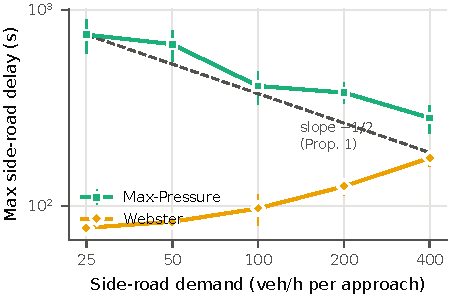
\includegraphics[width=0.48\textwidth]{figures/fig5_proposition.pdf}
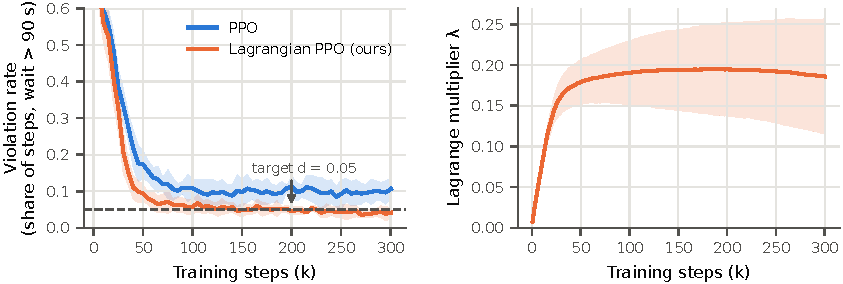
\includegraphics[width=0.48\textwidth]{figures/fig2_training.pdf}
\caption{Left: Proposition~\ref{prop:starve} in SUMO. Right: training curves (5 seeds).}
\label{fig:prop}\label{fig:training}
\end{figure}
\end{document}
